% orx-figures TikZ architecture, v6. Final printed size: 6.75 x 5.0625 in.
% Module positions are relative; local coordinates are used only inside icons.
\documentclass[border=0pt]{standalone}
\usepackage{fontspec}
\setmainfont{texgyreheros-regular.otf}[BoldFont=texgyreheros-bold.otf,ItalicFont=texgyreheros-italic.otf]
\setsansfont{texgyreheros-regular.otf}[BoldFont=texgyreheros-bold.otf,ItalicFont=texgyreheros-italic.otf]
\setmonofont{Inconsolatazi4-Regular.otf}[BoldFont=Inconsolatazi4-Bold.otf]
\usepackage{amsmath,fix-cm,fontawesome5,tikz}
\usetikzlibrary{arrows.meta,positioning,fit,backgrounds,calc,shapes.geometric}
\definecolor{ink}{HTML}{000000}
\definecolor{blue}{HTML}{245CA6}
\definecolor{bluefill}{HTML}{D8E8FA}
\definecolor{teal}{HTML}{087D83}
\definecolor{tealfill}{HTML}{D3EEEA}
\definecolor{amber}{HTML}{B67516}
\definecolor{amberfill}{HTML}{FFE7BB}
\definecolor{muted}{HTML}{536174}
\newcommand{\bodyfont}{\sffamily\fontsize{7.3}{9}\selectfont}
\newcommand{\smallfont}{\sffamily\fontsize{7}{8.5}\selectfont}
\newcommand{\headingfont}{\sffamily\bfseries\fontsize{8.2}{9.7}\selectfont}
\newcommand{\codefont}{\ttfamily\fontsize{7.5}{9.1}\selectfont}
\newcommand{\dd}{{\sffamily Δ}D}
\newcommand{\rulearrow}{\tikz[baseline=-.35ex]{\draw[double distance=.35pt,
  -{Implies[length=1.2mm,width=1.8mm]},line width=.35pt,draw=ink] (0,0)--(3mm,0);}}
\tikzset{
  orx/.style={font=\bodyfont,text=ink,line width=.65pt,
    >={Stealth[length=1.6mm,width=1.12mm]}},
  box/.style={draw=black,fill=bluefill,rounded corners=1.05mm,
    inner sep=0pt,outer sep=0pt,anchor=north west,line width=1pt},
  white/.style={box,fill=white,line width=1pt},
  runtime/.style={box},
  artifact/.style={box,draw=black,fill=tealfill},
  external/.style={box,draw=black,fill=amberfill},
  heading/.style={font=\headingfont,inner sep=0pt,anchor=north west},
  label/.style={font=\smallfont,inner sep=0pt,anchor=north west},
  code/.style={font=\codefont,inner sep=0pt,anchor=north west,align=left},
  icon/.style={inner sep=0pt,text=black,font=\sffamily\fontsize{10}{10}\selectfont},
  flow/.style={->,draw=ink,line width=.8pt,rounded corners=.6mm},
  io/.style={<->,draw=ink,line width=.7pt},
}
\newcommand{\personicon}[2]{%
  \begin{tikzpicture}[x=1mm,y=1mm,line width=.75pt,draw=black]
    \filldraw[fill=#1!16] (0,2.8) circle (1.65);
    \filldraw[fill=#1!16,rounded corners=.4mm]
      (-3.9,-3.6) -- (-3.9,-1.9) .. controls (-3.9,.9) and (3.9,.9) ..
      (3.9,-1.9) -- (3.9,-3.6) -- cycle;
    #2
  \end{tikzpicture}}
\newcommand{\tableicon}{%
  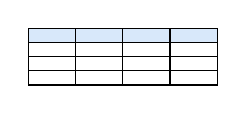
\begin{tikzpicture}[x=1mm,y=1mm,draw=black,line width=.45pt]
    \draw[fill=bluefill] (0,5.4) rectangle (24,7.2);
    \draw (0,0) rectangle (24,7.2);
    \foreach \x in {6,12,18} {\draw (\x,0) -- (\x,7.2);}
    \foreach \y in {1.8,3.6,5.4} {\draw (0,\y) -- (24,\y);}
  \end{tikzpicture}}
\newcommand{\treeicon}{%
  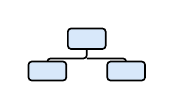
\begin{tikzpicture}[x=1mm,y=1mm,draw=black,line width=.6pt,rounded corners=.4mm]
    \draw (0,3.6) -- (0,2.2) -| (-5,1.3);
    \draw (0,2.2) -| (5,1.3);
    \draw[fill=bluefill] (-2.4,3.4) rectangle (2.4,6);
    \draw[fill=bluefill] (-7.4,-.6) rectangle (-2.6,1.8);
    \draw[fill=bluefill] (2.6,-.6) rectangle (7.4,1.8);
  \end{tikzpicture}}
\newcommand{\dbicon}[1]{%
  \begin{tikzpicture}[x=1mm,y=1mm,draw=black,line width=.6pt]
    \fill[bluefill] (-3.6,0) -- (-3.6,5) arc[start angle=180,end angle=0,x radius=3.6,y radius=.95]
      -- (3.6,0) arc[start angle=0,end angle=-180,x radius=3.6,y radius=.95];
    \draw (-3.6,5) -- (-3.6,0) arc[start angle=180,end angle=360,x radius=3.6,y radius=.95] -- (3.6,5);
    \draw[fill=bluefill] (0,5) ellipse[x radius=3.6,y radius=.95];
    #1
  \end{tikzpicture}}
\begin{document}
\begin{tikzpicture}[orx]
  \coordinate (origin) at (0,0);
  \node[box,fill=white,dash pattern=on 2mm off 1.1mm,line width=1pt,
    minimum width=149mm,minimum height=84.5mm,
    below right=1mm and 21mm of origin] (system) {};
  \node[heading,below right=2.1mm and 3mm of system.north west,
    font=\sffamily\bfseries\fontsize{10.4}{11.5}\selectfont]
    {Incremental Semantic View Maintenance System};
  \node[label,anchor=north east,below left=2.6mm and 3mm of system.north east,
    text=black] {Prototype};

  \node[artifact,minimum width=50mm,minimum height=35mm,
    below right=10mm and 3mm of system.north west] (spec) {};
  \node[icon,text=black,below right=2mm and 2mm of spec.north west,anchor=north west] {\faIcon{file-alt}};
  \node[heading,below right=2.1mm and 6.2mm of spec.north west]
    {Declarative Specification};
  \node[label,below right=6.5mm and 2mm of spec.north west,text=black]
    {Using Declarative Semantic Operator API};
  \node[label,font=\sffamily\bfseries\fontsize{7.2}{8.8}\selectfont,
    below right=10.2mm and 2mm of spec.north west] {Semantic view query};
  \node[white,draw=black,minimum width=46mm,minimum height=7.6mm,
    below right=13.6mm and 2mm of spec.north west] (querybox) {};
  \node[code,below right=2.3mm and 1.5mm of querybox.north west]
    {V = D.sem\_map("Extract ...")};
  \node[label,font=\sffamily\bfseries\fontsize{7.2}{8.8}\selectfont,
    below right=22.7mm and 2mm of spec.north west] {Physical storage specification};
  \node[white,draw=black,minimum width=46mm,minimum height=7mm,
    below right=26.1mm and 2mm of spec.north west] (storagecode) {};
  \node[code,below right=1mm and 1.5mm of storagecode.north west]
    {STORE V IN qdrant.memories\\KEY id; VECTOR embedding};

  \node[box,minimum width=38mm,minimum height=35mm,
    right=3mm of spec.north east,anchor=north west] (compiler) {};
  \node[heading,below right=2.1mm and 5.5mm of compiler.north west] (compilerheading) {Maintenance Compiler};
  \node[icon,anchor=east,left=.8mm of compilerheading.west,
    font=\sffamily\fontsize{8}{8}\selectfont] {\faCogs};
  \node[label,below right=6.4mm and 2mm of compiler.north west] {Apply and compose rules};
  \node[white,draw=black,minimum width=34mm,minimum height=23.5mm,
    below right=10.7mm and 2mm of compiler.north west] (rules) {};
  \node[code,below right=1.4mm and 1.4mm of rules.north west]
    {V = D.sem\_map(instr)\\
     \rulearrow\ V' = V.union(\\
     \hspace{1mm}\dd.sem\_map(instr))\\[2.1mm]
     V = D.sem\_filter(instr)\\
     \rulearrow\ V' = V.union(\\
     \hspace{1mm}\dd.sem\_filter(instr))};

  \node[artifact,minimum width=49mm,minimum height=35mm,
    right=3mm of compiler.north east,anchor=north west] (plan) {};
  \node[heading,below right=2.1mm and 5.5mm of plan.north west]
    (planheading) {Incremental Maintenance Plan};
  \node[icon,anchor=east,left=.8mm of planheading.west] {\faFileCode};
  \node[white,draw=black,minimum width=45mm,minimum height=23.5mm,
    below right=10.7mm and 2mm of plan.north west] (plancode) {};
  \node[code,below right=1.4mm and 1.2mm of plancode.north west]
    {Inputs: \dd, V\\[2.2mm]
     V' = V.union(\\
     \hspace{1.2mm}\dd.sem\_map("Extract ..."))\\[2.2mm]
     Output: V'};

  \node[inner sep=0pt,left=6.5mm of spec.west] (developer)
    {\personicon{blue}{\node[fill=white,draw=black,rounded corners=.4mm,
      inner sep=.5mm,text=black,font=\sffamily\bfseries\fontsize{7}{7}\selectfont]
      at (2.6,-3) {\textless/\textgreater};}};
  \node[heading,anchor=north,below=1.5mm of developer.south,text=black] {Developer};
  \draw[flow,draw=black] (developer.east) -- (spec.west);
  \draw[flow] (spec.east) -- (compiler.west);
  \draw[flow] (compiler.east) -- (plan.west);

  \node[runtime,minimum width=112mm,minimum height=24mm,
    below right=4mm and 31mm of spec.south west] (executor) {};
  \node[heading,anchor=north,below=1.8mm of executor.north,text=black,
    font=\sffamily\bfseries\fontsize{10}{11}\selectfont] {Incremental Executor};
  \node[white,draw=black,minimum width=30mm,minimum height=15mm,
    below right=7mm and 2mm of executor.north west] (execution) {};
  \node[heading,anchor=north,below=1.3mm of execution.north,
    font=\sffamily\bfseries\fontsize{7.6}{9.2}\selectfont] {Query Plan Execution};
  \node[inner sep=0pt,anchor=north,below=6.4mm of execution.north] {\treeicon};
  \node[white,draw=black,minimum width=44mm,minimum height=15mm,
    right=2mm of execution.north east,anchor=north west] (views) {};
  \node[heading,anchor=north,below=1.1mm of views.north,align=center,
    font=\sffamily\bfseries\fontsize{7.8}{8.7}\selectfont]
    {Materialized Semantic Views};
  \node[inner sep=0pt,anchor=north,below=6.6mm of views.north] {\tableicon};
  \node[white,draw=black,minimum width=30mm,minimum height=15mm,
    right=2mm of views.north east,anchor=north west] (intermediate) {};
  \node[heading,anchor=north,below=1.3mm of intermediate.north,
    font=\sffamily\bfseries\fontsize{7.6}{9.2}\selectfont] {Intermediate Results};
  \node[inner sep=0pt,anchor=north,below=6.6mm of intermediate.north] {\tableicon};
  \draw[flow] (plan.south) -- (plan.south |- executor.north)
    node[midway,right=1mm,font=\smallfont,fill=white,inner sep=.3mm] {Execute};

  \node[box,draw=black,fill=none,minimum width=28mm,minimum height=11mm,
    left=4mm of executor.west,anchor=east] (input) {};
  \node[heading,anchor=center,text=black] at (input.center) {Input data ΔD};
  \node[inner sep=0pt] (enduser) at (developer.center |- input.center) {\personicon{teal}{}};
  \node[heading,anchor=north,below=1.5mm of enduser.south,text=black] {End User};
  \draw[flow,draw=black] (enduser.east) -- (input.west);
  \draw[flow,draw=black] (input.east) -- (executor.west);
  \node[box,minimum width=45mm,minimum height=6.5mm,
    below=6mm of execution.south,anchor=north] (adapter) {};
  \node[heading,anchor=center] at (adapter.center) {\textcolor{black}{\faPlug}\quad Engine Adapter};
  \node[box,minimum width=46mm,minimum height=6.5mm,
    below left=4mm and 0mm of executor.south east,anchor=north east] (connector) {};
  \node[heading,anchor=center,font=\sffamily\bfseries\fontsize{7.8}{9.4}\selectfont] at (connector.center)
    {\textcolor{black}{\faPlug}\quad Physical Storage Connector};
  \draw[io] (execution.south) -- (execution.south |- adapter.north);
  \draw[io] (connector.north) -- (connector.north |- executor.south);

  \node[external,minimum width=93mm,minimum height=23mm,
    below right=5mm and 1mm of system.south west] (engines) {};
  \node[heading,anchor=north,below=1.6mm of engines.north,
    font=\sffamily\bfseries\fontsize{9.2}{10}\selectfont]
    {\textcolor{black}{\faCubes}\quad Semantic Query Processing Engines};
  \node[white,draw=black,minimum width=36mm,minimum height=15mm,
    below right=6.2mm and 2mm of engines.north west] (lotus) {};
  \node[heading,anchor=north,below=1.1mm of lotus.north] {LOTUS};
  \node[label,anchor=north,below=4.8mm of lotus.north,align=center]
    {Proxy-model cascades\\Prompt / operator cache\\Prompt optimization (DSPy)};
  \node[white,draw=black,minimum width=50mm,minimum height=15mm,
    right=3mm of lotus.north east,anchor=north west] (docetl) {};
  \node[heading,anchor=north,below=1.1mm of docetl.north] {DocETL / MOAR};
  \node[label,anchor=north,below=4.8mm of docetl.north,align=center]
    {Operator Fusion / Split / Reordering\\Code generation\\Agentic Prompt Rewriting};
  \node[label,anchor=south east,above left=1.2mm and 2mm of engines.north east,
    text=black,font=\sffamily\itshape\fontsize{7}{8.5}\selectfont] {Examples};
  \node[external,minimum width=48mm,minimum height=37.2mm,
    right=4mm of engines.north east,anchor=north west] (storage) {};
  \node[heading,anchor=north,below=1.6mm of storage.north,
    font=\sffamily\bfseries\fontsize{9.2}{10}\selectfont] {Storage Backends};
  \node[inner sep=0pt,anchor=center] (vector)
    at ($(storage.north west)+(8mm,-11mm)$)
    {\dbicon{\draw[->] (-2.3,.1) -- (-2.3,3.8);\draw[->] (-2.3,.1) -- (2.3,.1);
    \foreach \x/\y in {-1.1/1,0/1.8,1.3/2.8} {\fill[black] (\x,\y) circle(.3);}}};
  \node[label,anchor=west,font=\sffamily\fontsize{7.8}{9.4}\selectfont]
    at ($(storage.north west)+(15mm,-11mm)$) {Vector DB (Qdrant)};
  \node[inner sep=0pt,anchor=center] (graph)
    at ($(storage.north west)+(8mm,-21mm)$)
    {\dbicon{\draw (-1.9,.8) -- (-.5,3.1) -- (1.9,1.3) -- (-1.9,.8);
      \foreach \x/\y in {-1.9/.8,-.5/3.1,1.9/1.3} {\filldraw[fill=white] (\x,\y) circle(.5);}}};
  \node[label,anchor=west,font=\sffamily\fontsize{7.8}{9.4}\selectfont]
    at ($(storage.north west)+(15mm,-21mm)$) {Graph DB (Neo4j)};
  \node[icon,anchor=center,font=\sffamily\fontsize{17}{17}\selectfont] (files)
    at ($(storage.north west)+(8mm,-31mm)$) {\faFolderOpen};
  \node[label,anchor=west,font=\sffamily\fontsize{7.8}{9.4}\selectfont]
    at ($(storage.north west)+(15mm,-31mm)$) {File System};
  \node[label,anchor=south east,above left=1.2mm and 2mm of storage.north east,
    text=black,font=\sffamily\itshape\fontsize{7}{8.5}\selectfont] {Examples};
  \draw[io] (adapter.south) -- (adapter.south |- engines.north)
    node[midway,left=1.2mm,font=\smallfont,fill=white,inner sep=.3mm] {Queries / results};
  \draw[io] (connector.south) -- (connector.south |- storage.north)
    node[midway,left=1.2mm,font=\smallfont,fill=white,inner sep=.3mm] {Reads / writes};
  \node[external,minimum width=93mm,minimum height=11.2mm,
    below=3mm of engines.south,anchor=north] (models) {};
  \node[heading,anchor=north,below=1mm of models.north]
    {\textcolor{black}{\faBrain}\quad Model Services};
  \node[label,below right=4.8mm and 2.4mm of models.north west]
    {\textbf{LLMs:} GPT-6-Astra, DeepSeek-Flash, Claude Sonnet 4.6};
  \node[label,below right=7.8mm and 2.4mm of models.north west]
    {\textbf{Embedding Models:} BGE-M3, text-embedding-3-small};
  \draw[io] (models.north) -- (engines.south);
  \pgfresetboundingbox
  \path[use as bounding box] (origin) rectangle ++(171.45mm,-128.5875mm);
\end{tikzpicture}
\end{document}
